\documentclass[
class = book,
zihao = -4,
font = noto,
paper = a4paper,
openany
]{easybook}

\usepackage{xju}
\newcommand{\ti}{Ti6Al4V}
%笔记
%先模仿,而后进行整改
\begin{document}
	\hypersetup{pdftitle=Ti-6Al-4V 钛合金热处理工艺的研究现状及进展,pdfauthor=田欣洋,pdfsubject={材料科学,金属学,钛合金},pdfkeywords={热处理,固溶,时效,组织},pdfstartview=FitB}
	\maketitle
	\frontmatter*[roman]

	\begin{abstract}
		\ti 合金又名TC4合金,拥有较好的塑韧性、耐热性、成形性、耐蚀性等,在机械、军事、航空航天等领域获得了极为广泛的应用。但TC4合金仍存在硬度较低、摩擦磨损系数高、耐磨性能差、较低的塑韧性和力学性能上的各向异性等缺点,制约了其进一步的应用。
%		初步撰写,模仿《TC4 钛合金热处理工艺的研究现状及进展——孟宪伟袁赵锦秀》
		本文阐述了TC4钛合金的热处理工艺研究现状,并分析了不同热处理制度对Ti6Al4V合金强度的影响,并解析了组织转变的机理,为工程应用提供了有价值的参考,最后提出了TC4钛合金热处理工艺的研究方向。\\

		\keywords{Ti-6Al-4V 钛合金;热处理;显微组织;力学性能;固溶;时效;现状}
	\end{abstract}

	\tableofcontents
	\mainmatter*
	\pagestyle{Xju}
\chapter{前言}
工业上一般根据$\beta $相稳定元素系数$K_{\beta}$来划分不同类型的钛合金,$K_{\beta}$是指合金中各$\beta $稳定元素与各自的临界浓度的比制之和,即:
$$
K_{\beta}=\frac{ C_{1} }{C_{k1}}+\frac{ C_{2} }{C_{k2}}+\frac{ C_{3} }{C_{k3}}+\cdots+\frac{ C_{n} }{C_{kn}}
$$
根据 $\beta$ 相稳定系数划分合金类型为:

\begin{table}[htbp]
	\centering
	\label{sec:sort}
	\caption{钛合金类型分类}
		\begin{tabular}{ccc}
			\toprule
			类型&$K_\beta$值&主要合金元素 \\
			\midrule
			 $\alpha$ 型& $0 \sim 0.07$&铝、锡、锆\\
			 近 $\alpha$ 型&$0.07 \sim 0.25$&铝、锡、锆与少量钒、钼、铌\\
			 $\alpha+\beta$ 型&$0.25 \sim 1.0$&以铝为主、以及其他少量$\beta$ 相稳定元素\\
			 近 $\beta$ 型&$1.0 \sim 2.8$&少量钒、钼、铌、钽、等\\
			$\beta$ 型&$ > 2.8 $&大量钒、钼、铌、钽、等\\
			\bottomrule
		\end{tabular}
\end{table}
其中$\alpha $+$\beta $型钛合金的特点是既有α稳定元素,又有β稳定元素,使α和β同 时 得 到 强 化 。β稳 定 元 素 加 入 量 为 4% ~6% ,目 的 是 为 了 获 得 足 够 数 量 的β相 ,以 改 善 合 金 的 成 形 塑 性 和 使 合 金 得 到热处理强化的能力,对其进行退火处理,所得到的室温组织为不同比例的$\alpha $和$\beta $相。$\alpha $+$\beta $型钛合金的强度和淬透性随着$\beta $相稳定元素含量增加而提高,其锻造和轧制等加工成型性能优于$\alpha $型、$\beta $型钛合金。从成分上来看,这类钛合金中的合金元素基本上是以铝为主要合金元素,$\beta $稳定化元素为辅助元素。这使得$\alpha $+$\beta $型钛合金组织变动的余地较为灵活,性能变动范围大,可以满足各种应用场合及工况要求\cite{TiandAl}。

我国用TC表示$\alpha $+$\beta $型双相钛合金,最常用的$\alpha $+$\beta $型钛合金包括TC4、TC6、TC12等,其中TC4钛合金(等轴马氏体型两相合金)作为做早被应用的钛合金,该合金以其优越的性能占据了钛工业的大量市场,现在占到 Ti 合金总产量的 50$ \%  $, 占到全部Ti 合金加工件的95$ \% $ 。

TC4钛合金具有较高的抗拉强度和抗疲劳强度、生物相容性好、耐高温、化学性质性质稳定、高硬度和良好的耐腐蚀性、弹性模量低、低密度等优良特性,在航空航天、汽车工业、医疗健康领域等领域得到了广泛应用,是目前应用最广泛的钛合金 。 但其室温塑性较低 , 加工硬化能力较差 , 冷加工成型困难。

 目前相关研宄中 , 提升 TC4钛合金室温塑性的手段包括添加合金元素、剧烈塑性变形和相变热处理等。 而近些年来国内对于\ti 合金的研究取得了许多成果\cite{tc42021}。但是大多数关于TC4钛合金热处理工艺研究现状的文章的表述并不太清楚,没有结合最新的计算机技术进行探讨,本文将从多个方面对TC4钛合金的研究现状以及发展方向进行一个科学全面富有前瞻性的展望。

现阶段\ti 合金的热处理工艺主要集中在如下三个方面:
\begin{enumerate}
	\item 固溶处理:实施固溶处理工艺,是为了得到等轴稳定的$\alpha $相、马氏体弥散的$ \alpha ^{'} $相、亚稳定状态的$\beta $相,等轴的$\alpha $相能够让合金的力学性能得到综合性的提升,马氏体弥散的$ \alpha ^{'} $相能够让合金,在强度、硬度上得到提高,塑性、韧性被降低\cite{gurong2002}。
	\item 时效处理:有研究\cite{timing}发现,次生的$\alpha $相体积分数在TC4钛合金中,会对屈服强度产生很大的影响。在条件相等的情况之下,时效温度越低组织越小,时效温度高低组织越大。研究人员主要是通过控制参数,来影响对次生$\alpha $相的含量,从而来实现TC4钛合金在力学的性能上得到更好的提升。
	\item 深冷处理:深冷处理是近些年来新兴的一种处理工艺,其可以对金属内部的组织进行改善,在进行深冷处理的时候操作比较方便,对环境也不会造成太大的污染,并且能够让在热处理之后残留的奥氏体被清除掉。实验研究发现,原始的$\beta $相会在深冷处理的过程当中,逐渐的向$\alpha $、相去转变,残余应力在组织中会变少,与此同时网篮状组织的增加,会让TC4钛合金的韧性、强度、塑性,在组织上的性能得到提高。
\end{enumerate}

%
\section{参考甲}
\subsection{试样}
拉伸试样的尺寸参数:厚度是7毫米,宽度(20±0.05)毫米,长度(60 + 0.5)毫米。夹紧端是50毫米的长度。曲率之间的平行段长度和夹紧端是大于或等于12。拉伸试样的总长度大于184mm。应变 率 是 0.003 $ s^{-1} $。
\newpage
\subsection{机理}
%The α-phase is the substrate phase of (α+β)-titanium alloy. The number, shape and size of α-phase determine directly the property of (α+β)-titanium alloy. In the two-phase region, (α+β)-phase is gotten from the heat treatment with different holding time and temperatures. The temperature is below the phase transition temperature. The main characteristics of (α+β)-phase microstructure are irregular shape of grains, continuous and discontinuous α-phase on the grain boundary, and many small secondary α-phases. The punctate, spherical, flakiness and short rod α-phase exists in intragranular[22]. However, all (α+β)-phase will be converted into β-phase when the heating temperature is higher than phase transition temperature. The size and shape of grains are not identical. They are quadrilateral, pentagon and hexagon.
%
%Solution and aging can eliminate or reduce α-phase of continuous grain boundary. They can improve significantly the tensile and fatigue strength. But the plasticity will decrease a little. Solution and aging treatment can improve obviously the fatigue strength. The more stable β-phase of alloy, the more β-phase metastable after quenching. Then the effect of aging strengthening is better. Maximum effect will be gotten when the temperature of β stable element reaches CK value. Strengthening effect decreases with the rise of β-phase. That causes precipitation of aging β-phase metastable and the number of α-phase declines. Ti6Al4V alloy is (α+β)-phase alloy. The microstructure and mechanical properties can be improved by the solution and aging heat treatment, and then better comprehensive properties can be obtained [23,24].
\begin{table}[htbp]
	\centering
	\label{sec:myHT}
	\caption{\ti 热处理工艺与性能汇总表\cite{LiuWanYingBuTongReChuLiGongYiDuiTi6Al4VTaiHeJinWeiGuanJieGouHeLiXueXingNengYingXiangYingWen2017}}
	\resizebox{\textwidth}{!}{
		\begin{tabular}{cccccc|cccc}
			\toprule
			固溶温度/℃ &用时/h & 冷却 & 时效温度/\textcelsius &用时/h & 冷却&屈强/Mpa&抗拉强度/Mpa&延伸率$\%  $&冲击韧性$ A_k /j \cdot cm^{-2} $ \\
			\midrule
			\hot{热轧}{——}{——}{——}{——}{——}{700}{790}{12.81}27.60\\
			\hot{920}{1}{WQ}{450}{4}{AC}{890}{1000}{15.00}40.00\\
			\hot{920}{1}{WQ}{500}{4}{AC}{960}{1070}{13.82}38.21\\
			\hot{960}{1}{WQ}{450}{4}{AC}{960}{1050}{15.48}43.64\\
			\hot{960}{1}{WQ}{500}{4}{AC}{1050}{1120}{16.28}46.22\\
			\hot{1000}{1}{WQ}{450}{4}{AC}{1000}{1100}{12.08}33.05\\			\hot{1000}{1}{WQ}{550}{4}{AC}{1020}{1100}{10.23}30.63\\
			\bottomrule
		\end{tabular}
	}
\end{table}
\begin{figure}[h!]
	\centering
	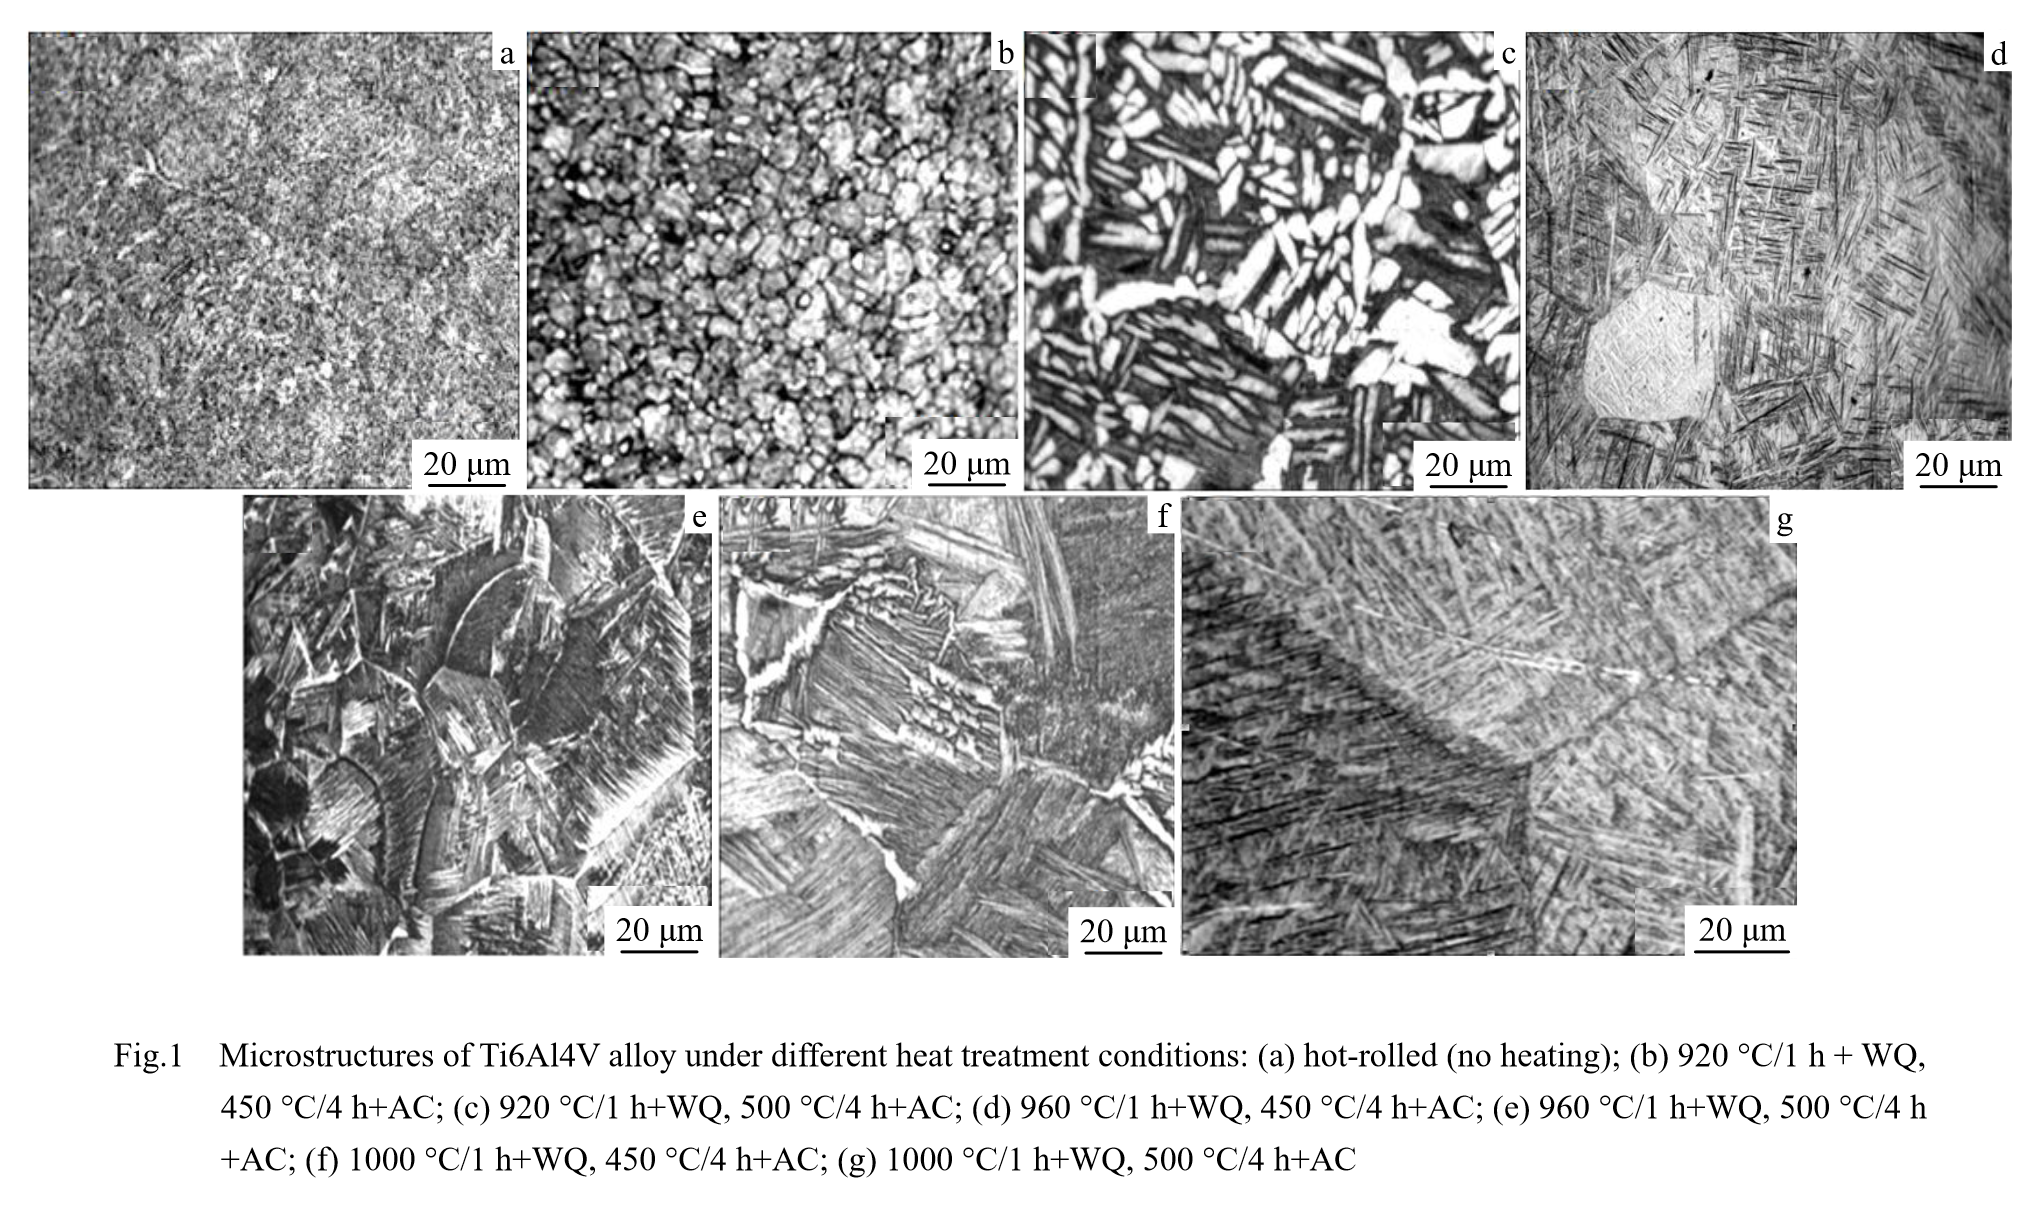
\includegraphics[width=0.8\linewidth]{金相_甲}
	\caption[参考一]{组织金相图}
	\label{fig:}
\end{figure}
% TODO: \usepackage{graphicx} required
\begin{figure}[h!]
	\centering
	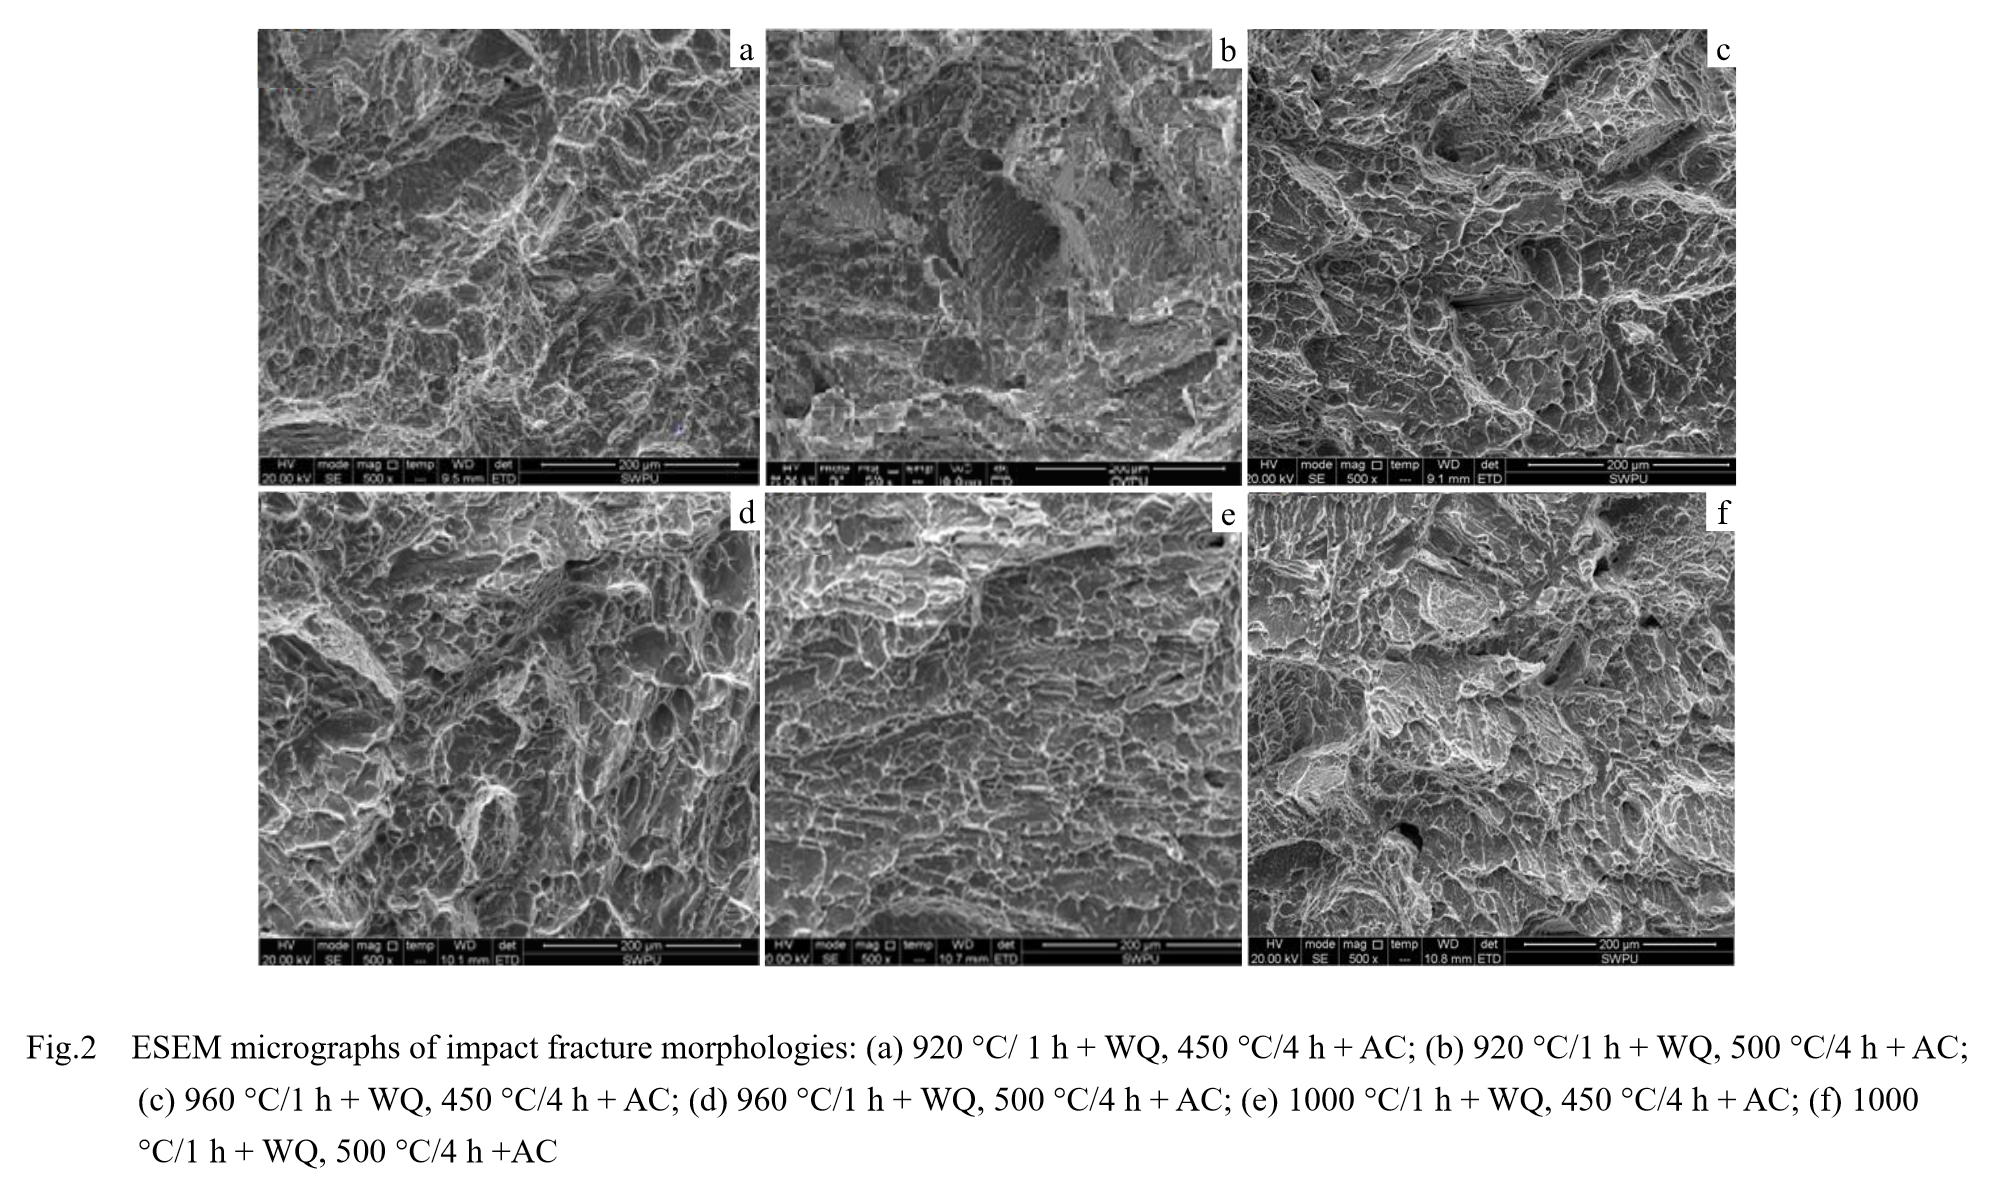
\includegraphics[width=0.8\linewidth]{其他_甲}
	\caption{断口形貌}
	\label{fig:}
\end{figure}
%
\section{参考乙}
\begin{table}[htbp]
	\centering
	\label{sec:my1HT}
	\caption{\ti 热处理工艺与性能汇总表\cite{RanXingGuRongWenDuDuiTi6Al4VELITaiHeJinXianWeiZuZhiJiXingNengDeYingXiang2021}}
	\resizebox{\textwidth}{!}{
		\begin{tabular}{ccccccccc}
			\toprule
			固溶温度/℃ &用时/h & 冷却 & 时效温度/\textcelsius &用时/h & 冷却&屈强/Mpa&抗拉强度/Mpa&延伸率$\%  $\\
			\midrule
			\hot{952}{2}{WQ}{730}{4}{AC}{846}{915}{16.80}\\
			\hot{967}{2}{WQ}{730}{4}{AC}{801}{875}{11.2}\\
			\hot{997}{2}{WQ}{730}{4}{AC}{792}{861}{9.6}\\
			\hot{1012}{2}{WQ}{730}{4}{AC}{775}{843}{8.2}
			\bottomrule
		\end{tabular}
	}
\end{table}
\begin{figure}[h!]
	\centering
	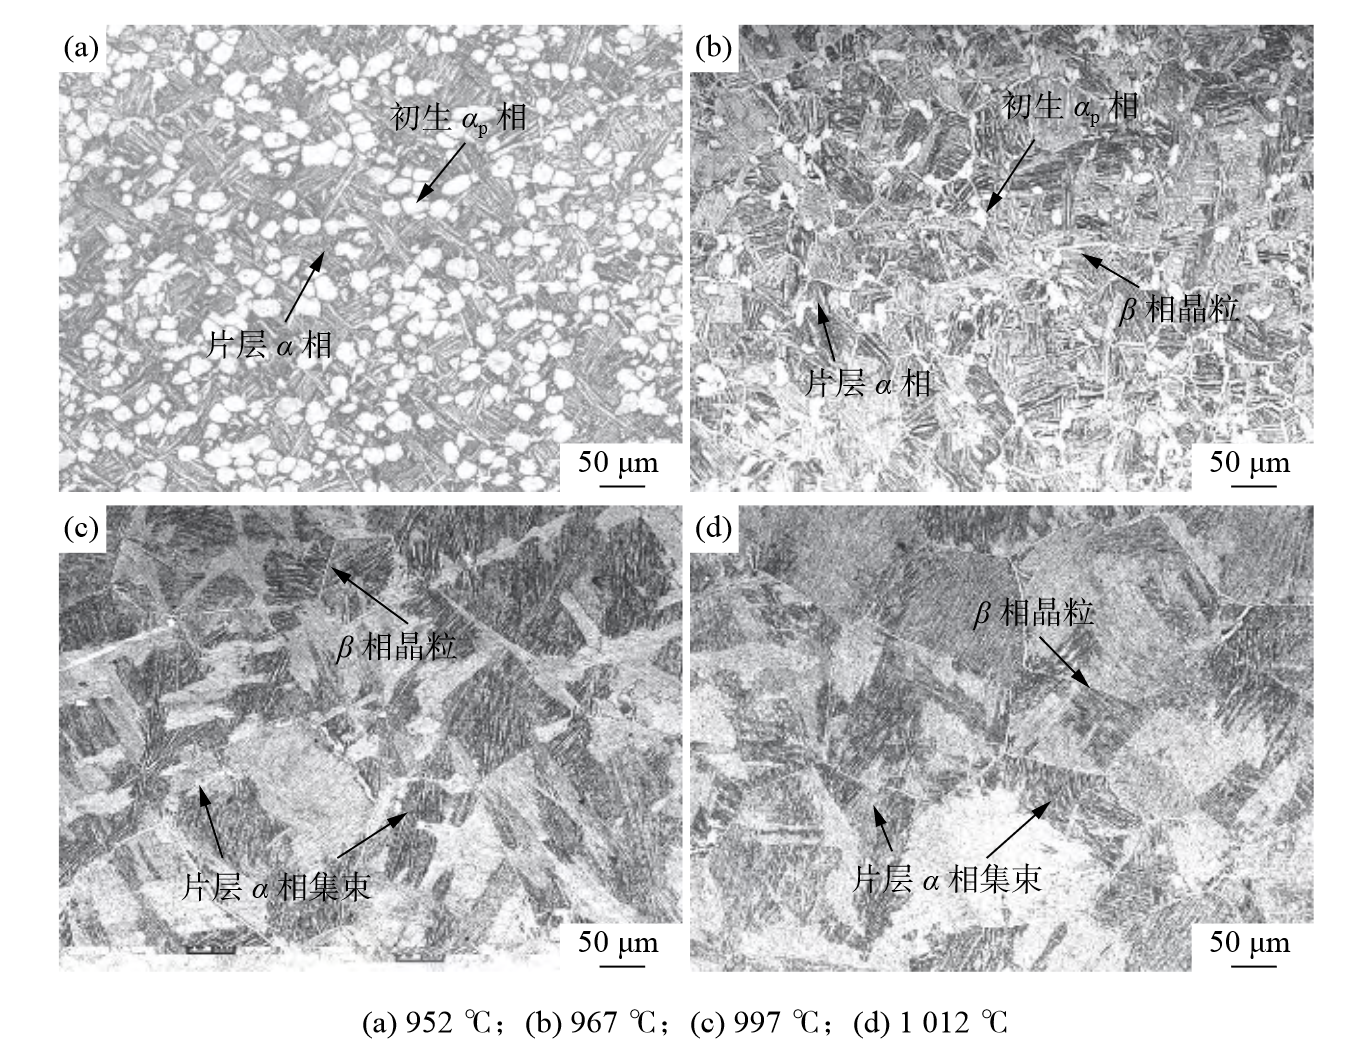
\includegraphics[width=0.7\linewidth]{金相_乙}
	\caption{金相组织}
	\label{fig:}
\end{figure}
% TODO: \usepackage{graphicx} required
\begin{figure}[h!]
	\centering
	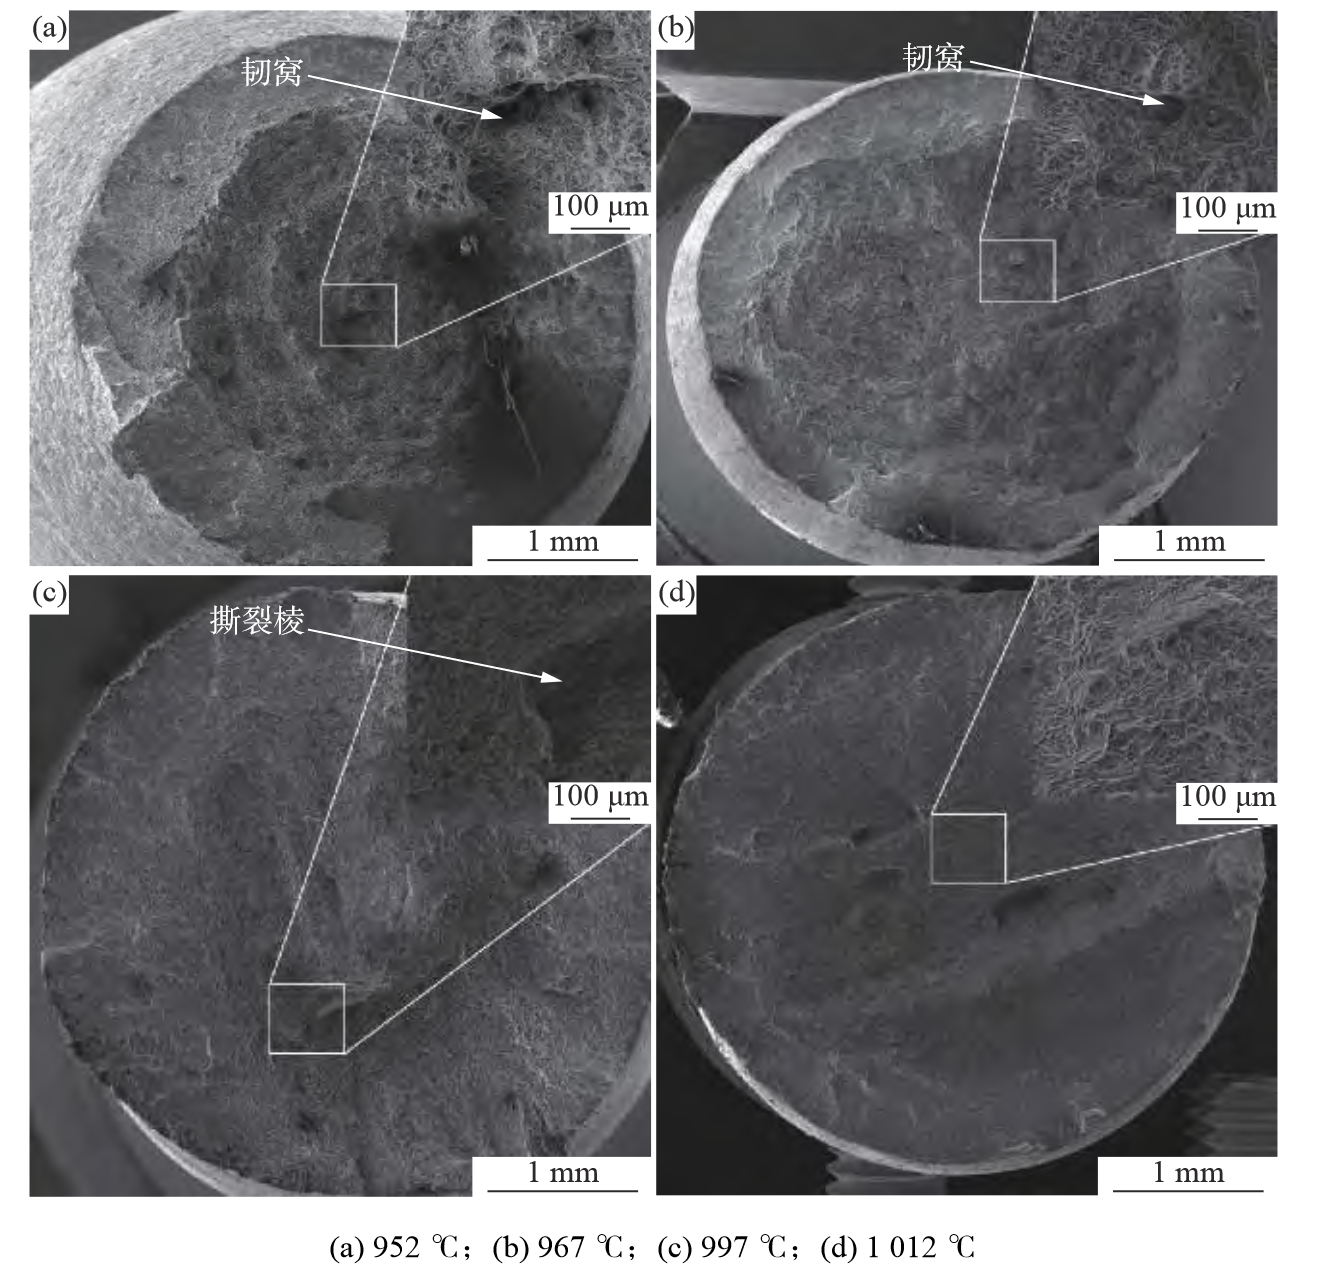
\includegraphics[width=0.7\linewidth]{断口_乙}
	\caption{断口形貌}
	\label{fig:}
\end{figure}


%\chapter{热处理工艺对显微组织转变的影响}
\section{实验用TC4合金的特点}
从制备方式上来看。近些年相关热处理实验中的TC4钛合金大多数是由{多次真空自耗电弧炉熔炼}\cite{renchiqiangGurongshixiaoduiTC4taihejinxianweizuzhihelixuexingnengdeyingxiang2022,ranxingGurongwenduduiTi6Al4VELItaihejinxianweizuzhijixingnengdeyingxiang2021,lilouGurongshixiaoduiTC4hejinzuzhiyujixiexingnengdeyingxiang2014,jingranGurongshixiaoduiTC4hejinzuzhiyuxingnengdeyingxiang2018}而成,其余的是通过粉末冶金\cite{zhanghaoyinGurongShixiaoduiTC4taihejinzuzhihelixuexingnengdeyingxiang2014,xujianGurongshixiaogongyiduiTC4taihejinzuzhijixingnengdeyingxiang2014}的方式来制备TC4,此外还有一小部分用的是热轧合金\cite{LiuWanYingBuTongReChuLiGongYiDuiTi6Al4VTaiHeJinWeiGuanJieGouHeLiXueXingNengYingXiangYingWen2017}、电子束选区熔化合金\cite{leijunleDianzishuxuanquronghuachengxingTC4hejinxianweizuzhiyuxingnengdeyanjiujinzhan2022}、商用棒状TC4合金\cite{luyuanyuanShixiaochuliduiTC4taihejinweiguanzuzhihelixuexingnengdeyingxiang2019,baoxuechunRechuligongyiduiTC4taihejinzuzhihelixuexingnengdeyingxiang2019}等。其中真空自耗电弧炉熔炼得到的合金强度普遍较高,而粉末冶金法虽然工艺复杂,但其得到的组织晶粒细小、成分偏析少、机加工量减小,是TC4合金制备的新趋势。

从化学成分上来看。标准的TC4钛合金成分有国家标准:
\begin{table}[htbp]
	\centering
	\label{sec:mytc4chem}
	\caption{TC4合金化学成分的国家标准}
	\begin{tabular}{cccccccc}
		\toprule
		元素($ \% $) & Al & V &Fe &C& O& N &H \\ \midrule
		标准要求 &$ 5.5\sim 6.75 $ & $ 3.5\sim 4.5 $&$ \le 0.30 $ & $ \le 0.05 $&$ \le 0.20 $&$ \le 0.03$ &$ \le 0.015 $  \\ \bottomrule
	\end{tabular}
\end{table}
%开始废话填充模式。2023-1-9-13:05


本文统计了近年\ti 钛合金热处理研究方面的近十多篇文献,发现不同实验者在试验中用到的合金成分都有所差异,如\ref{sec:mytc4ave}所示。其中Al元素的含量差异较大,从$ 5.65\% $到$ 6.4\% $不等,v元素的含量差异较小,都在$ 3.97 \%$到$ 4.25\% $范围之间,其余的非主要的杂质元素成分如Fe、C、N、O等的含量也有不同,总的来讲含量都在国标的范围之内。
\begin{table}[htbp]
	\centering
	\caption{不同实验者所用的TC4合金元素统计}
	\label{sec:mytc4ave}
	\begin{tabular}{ccccccccc}
		\toprule
元素($ \% $)& Ti  & Al & V &Fe &C& N& O &H \\ \midrule
平均值 & 89.455 & 6.118 & 4.086 & 0.102 & 0.028 & 0.039 & 0.164 & 0.007 \\
方差 & 0.147 & 0.253 & 0.104 & 0.074 & 0.019 & 0.078 & 0.060 & 0.015 \\
标准差 & 0.022 & 0.066 & 0.011 & 0.006 & 0.000 & 0.006 & 0.004 & 0.000 \\
		\bottomrule
	\end{tabular}
\end{table}
从强度上来看,大多数试样的抗拉强度在850Mpa以上,屈服强度在830Mpa以上,强度普遍较低。在经过固溶、时效等热处理方式处理过后,试样的抗拉强度与屈服强度升到了900Mpa与1200Mpa之间。其中,最高的强度是任驰强等\cite{renchiqiangGurongshixiaoduiTC4taihejinxianweizuzhihelixuexingnengdeyingxiang2022}在954℃/60min(水冷,10秒)+550℃/300min(AC)方式下得到的组织,其抗拉强度$ \sigma_m $达到了1177Mpa,屈服强度为$ \sigma_{0.2} $为1061Mpa,可见热处理对于组织的优化还是很可观的。
\begin{table}[htbp]
	\centering
	\caption{TC4合金力学性能的国家标准}
	\label{sec:mytc4machin}
	\begin{tabular}{cccc}
		\toprule
		力学性能& 抗拉强度$Mpa  $& 屈服强度$ Mpa $&断后伸长率$ \% $\\ \midrule
		标准值 &$ \ge 895 $&$ \ge 830 $&$ \ge 10 $ \\ \bottomrule
	\end{tabular}
\end{table}

\begin{figure}[h!]
	\centering
	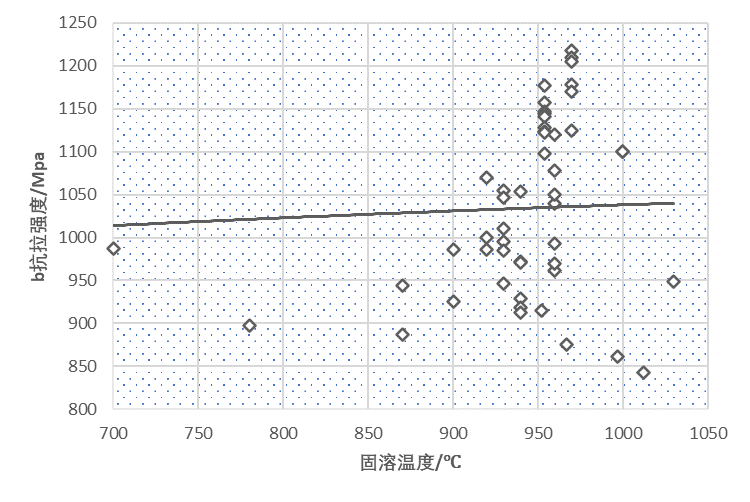
\includegraphics[width=0.7\linewidth]{固溶温度与抗拉强度}
	\caption{固溶温度与抗拉强度}
	\label{fig:gurongandstrength}
\end{figure}

\begin{figure}[h!]
	\centering
	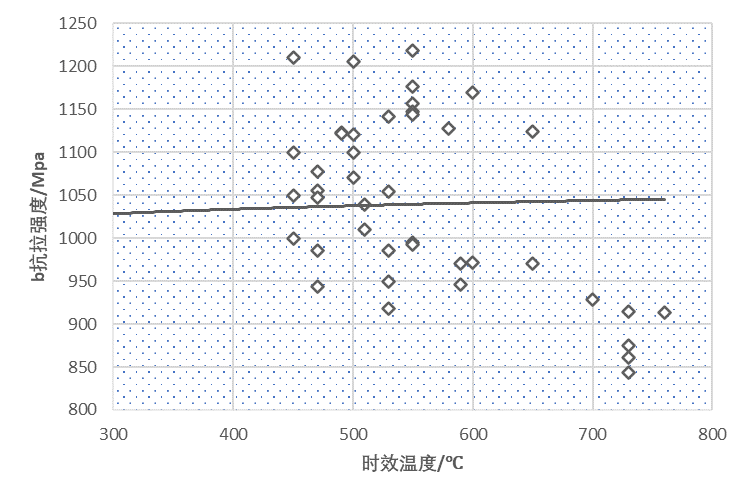
\includegraphics[width=0.7\linewidth]{时效温度与抗拉强度}
	\caption{时效温度与抗拉强度}
	\label{fig:shixiaoandstrength}
\end{figure}

\begin{figure}[h!]
	\centering
	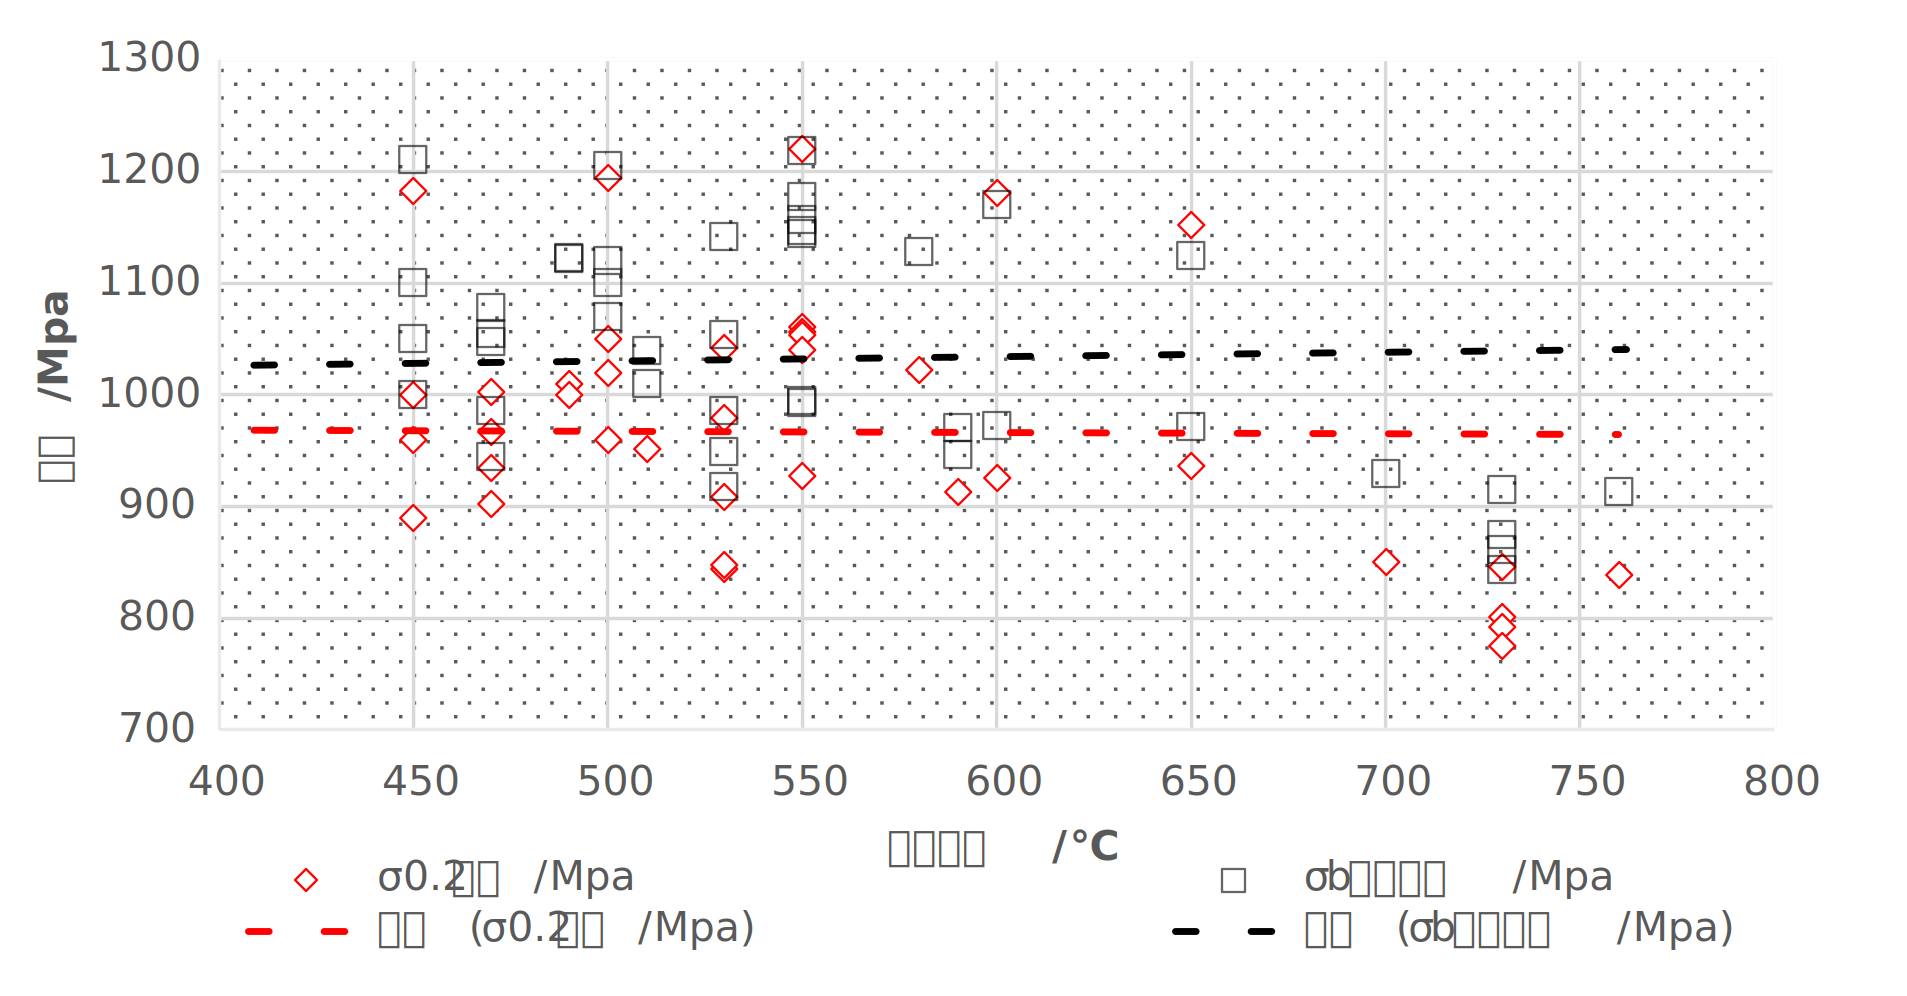
\includegraphics[width=0.7\linewidth]{时效温度与抗拉屈服强度}
	\caption{时效温度与抗拉屈服强度}
	\label{fig:时效温度与抗拉屈服强度}
\end{figure}



%	电 子 束 选 区 熔 化 技 术 ( Electron Beam Selective Melting,EBSM) 能量大、效 率高,粉末床 可 预 热, 制 件 热 应 力 小, 材 料 适 应 性 广,特别适于一 些 难 加 工、 脆 性 材 料
%دسسداسدسقىكىاكسىاكقھسسىكدقھسقكاھبكقسا
%سدبھقكساھبساھسفھسلكان
%ھساھسناھس
%اھسا
%ھساھساھسسدددددددددددددددددددددددددددددد
%ھسھھھ
%چچچچچچچچچچچچچچچچچۋدساسداسد

%材料的化学成分为:

%试样的尺寸为

%拉伸试验的参数为
\section{组织组成}
对于固溶处理过程,一般出现的组织为典型双态组织:球状的初生$ a_p $相、板条状a相、细小的b相转变组织以及部分粗大的b相转变组织\footnote{取向越无序、性能越差,最佳组织为\textbf{板条状α相组织之间分布着较为细小的β相转变组织}、\textbf{越粗大、取向越不规律}。则性能越差}。\cite{zhanghaoyinGurongShixiaoduiTC4taihejinzuzhihelixuexingnengdeyingxiang2014}固 溶 温 度 对 Ti6Al4V ELI钛合金显微组织形貌的影响主要在于 初生$ α_p $相含量、片层α相厚度以及β晶粒尺寸,其中粗大的初生$ α_p $相组织,对性能的影响较大,是不利因素;片层状α相是有利组织,可以很好地提高组织的的强度\cite{ranxingGurongwenduduiTi6Al4VELItaihejinxianweizuzhijixingnengdeyingxiang2021}。


\begin{figure}[h!]
	\centering
	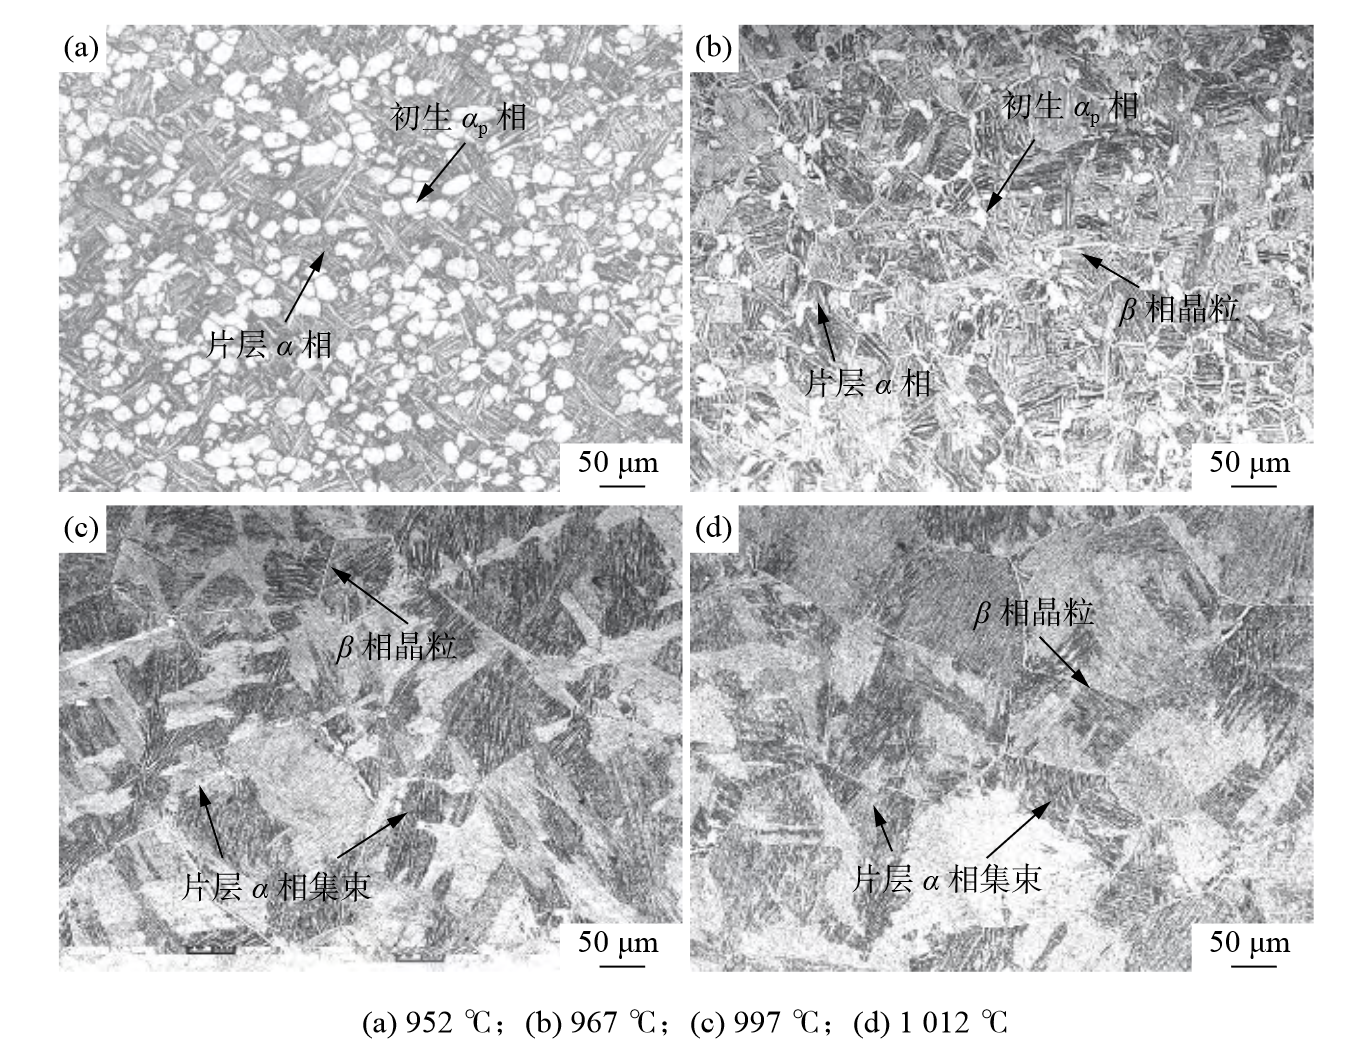
\includegraphics[width=0.7\linewidth]{金相_丙}
	\caption{不同固溶温度下TC4合金的显微组织}
	\label{fig:}
\end{figure}


总的来讲,固溶的作用是将粗大的双态组织均匀化,减小不同相之间的取向差异,从性能上来看,得到恰当成分的b相最有利于强度。

对于淬火过程,部分b相,转变成了a'相与a"相。

对于时效处理过程,出现的组织为a'相,a'相脱溶出来的等轴a相与b相、变粗大的a相与b相\footnote{固溶后钛合金中马氏体仍保持α相 软 而 韧 的 性 能,在随后进行的时效强化使得马氏体分解,获 得 弥 散 的α+β组织,从而进一步提高其抗拉强度。 随 着 时 效 温度的升高,伸长率逐 渐 上 升,但是抗拉强度则呈下降 趋势。}。\cite{zhanghaoyinGurongShixiaoduiTC4taihejinzuzhihelixuexingnengdeyingxiang2014}时效的作用就是将固溶后得到的亚稳定组织低温热处理, 促使亚稳定组织 β 相、α′相及 α′′相转变为细小、稳定 的等轴组织与片层组织以起到弥散强化作用。

\section{研究现状与展望}
 鲁媛媛,马保飞等人研究发现在时效温度为450、500和550℃时初生$\alpha $相的含量随温度升高逐渐增加;而在时效温度为600℃和650℃条件下初生$\alpha $相含量因高温溶解而明显减少, $\beta $相尺寸相应增大。当时效温度为550℃时, 所得钛合金的显微组织最佳\cite{timing}。



\chapter{固溶处理}
钛合金经过固溶处理后,能够改善其力学性能、激光切割加工性能以及耐热性能等,然而固溶处理温度的选择对于固溶效果影响非常大。如果固溶温度过低,无法达到充分的原子互溶,难以获得完全的β相,导致性能提高有限;如果固溶温度过高,会引起粗化效应,导致材料强度降低。

对于TC4钛合金来说,最佳的固溶温度范围在950-1000°C,这一温度范围可以使其达到最佳的综合性能。在这一温区内,可以基本实现β转变,而不会引起明显的粒度粗化。1000°C左右的固溶温度,可以达到$ 52-55\% $ 的β转变率,同时维持较小的平均β晶粒尺寸,这使TC4钛合金具有最佳的综合力学性能和韧性。

因此,选择适宜的固溶温度和保温时间是获得TC4钛合金优异性能的关键所在。固溶温度的精确控制,既需要严格的温度监控,也需要严格控制热处理设备的加热速率。只有在保持严格控制下,才能使TC4钛合金达到均匀的微观组织和最佳的综合性能。

%\chapter{热处理工艺对力学性能的影响}
\section{相变点与固溶温度的选择}
\subsection{相变点的计算}
通过合金元素的含量进行计算\footnote{《基于二元相图精确计算钛合金α+β/β相变点》}:
\begin{figure}[h!]
	\centering
	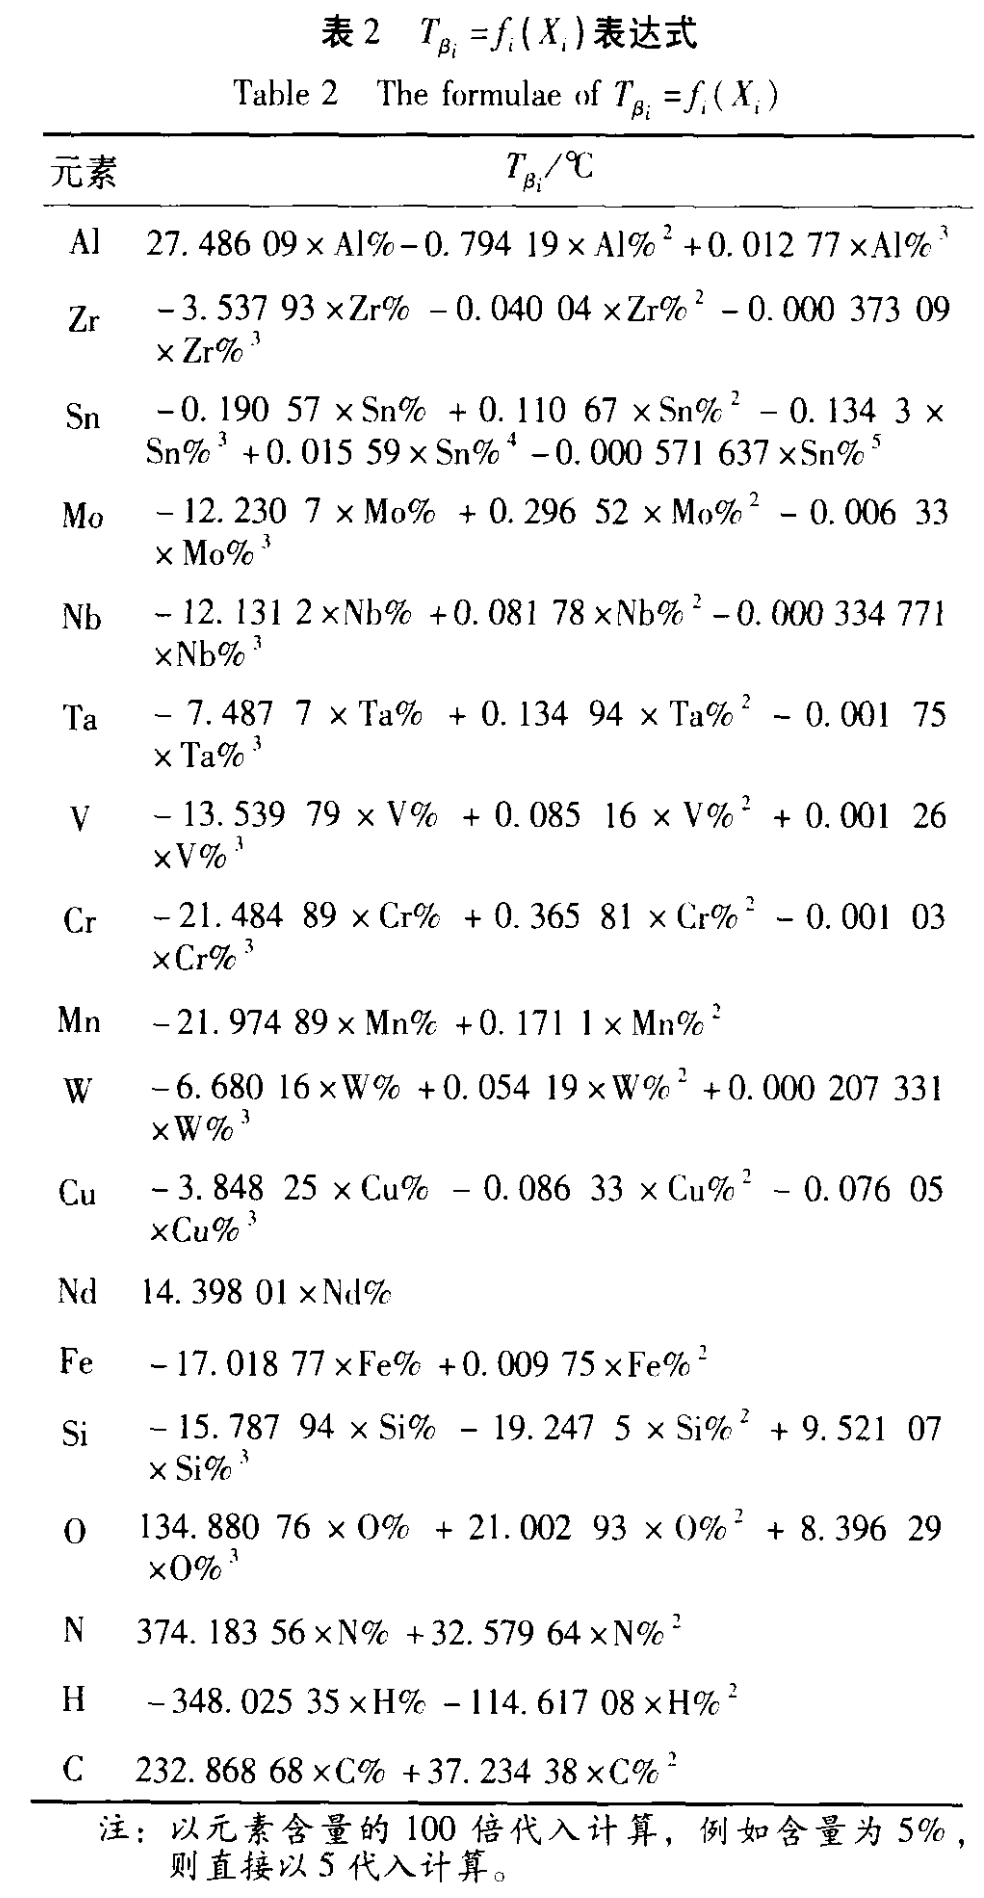
\includegraphics[width=0.8\linewidth]{相变点计算}
	\caption{相变点计算}
	\label{fig:keypoint}
\end{figure}

\chapter{时效处理}





经过调研发现,在大多数实验中当固溶温度选取在低于$ \beta $相变温度50度左右时,得到的性能最好。
\section{TC4合金性能与热处理制度的关系}

\section{研究现状与展望}
 刘婉颖、林元华等人通过实验发现:在960 ℃/1 h + WQ进行固溶处理和500 ℃/4 h + AC下进行时效处理得到的\ti 具有最佳的力学性能\cite{960500};陈冠宇通过实验表明,在850℃进行退火处理时,在600℃进行时效处理可以使合金得到更好的耐腐蚀性能\cite{1200};李宸宇证明\ti 合金在900℃空冷固溶两小时在530℃时效四小时后具有更好的强硬度,而且固溶后冷速越快,合金的强硬度越高、塑韧性越差\cite{900}。%第46页

%\chapter{发展趋势}

%\chapter{结论}
	\begin{enumerate}
		\item 对于组织
		\item 对于力学性能
		\item 对于其他性能
	\end{enumerate}


	\backmatter
	\listoffigures
	\listoftables
	\clearpage
	\phantomsection
	\addcontentsline{toc}{chapter}{参考文献}
	\bibliography{modern}
\end{document}


